\section{Overview}
``Angle Meter'' is a very simple Android app developed using the Eclipse ADT plugin and the 2.3 Android-SDK version.
It's intended use is the measuring of inclination angles (relative to the horizontal or vertical line) of flat surfaces.

\section{UML}
Here we have the UML diagram of the system:
\\
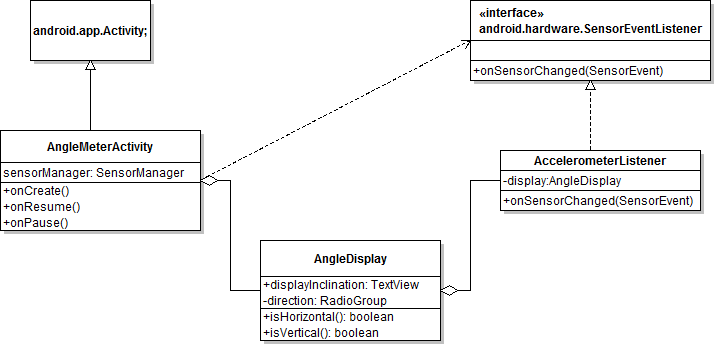
\includegraphics[scale=0.5]{images/UML.png} \\
\\

\section{Code}

\lstset{language=Java, caption=Initialization of the sensor and attaching the listener; lori.sma.AngleMeterActivity,
label=onChange}
\begin{lstlisting}
  private void initAccelerometer() {
    AngleDisplay display = new AngleDisplay();
    this.accelerometerListener = new AccelerometerListener(display);
    this.sensorManager = (SensorManager) this.getSystemService(
        Context.SENSOR_SERVICE);
    Sensor defSensor = this.sensorManager.getDefaultSensor(
        Sensor.TYPE_ACCELEROMETER);
    this.sensorManager.registerListener(this.accelerometerListener, 
        defSensor, SensorManager.SENSOR_DELAY_NORMAL);
  }
\end{lstlisting}


\lstset{language=Java, caption=The brains of the app from lori.sma.AccelerometerListener, label=onChange}
\begin{lstlisting}
 public void onSensorChanged(final SensorEvent event) {
    final Sensor acceletometer = event.sensor;

    if (acceletometer.getType() != Sensor.TYPE_ACCELEROMETER) {
      return;
    }
    float[] rotationMatrix = this.calculateRotationMatrix(event.values);
    double angle = this.calculateAngle(rotationMatrix);
    String toDisplay = AccelerometerListener.NUMBER_FORMAT.format(angle);
    this.display.displayInclination.setText(toDisplay);
  }
\end{lstlisting}

\section{Encountered Obstacles}

The initial design of the app was to add the ability to measure linear distances; e.g. move the phone against a
quasi-flat surface and have it tell you the length.

My plan was to use the GPS to get the altitude relative to the Earth's core so I could get a precise measurement of
gravity; then, subtract that from the acceleration values given by the accelerometers of the phone, thus obtaining
values only for the acceleration caused by the movement.

One can easily determine distance by integrating the acceleration twice. The problem is that the error in the data
provided by the accelerometer causes too much drift during integration; as ilustrated by this talk:
 \url{http://www.youtube.com/watch?v=C7JQ7Rpwn2k} - David Sachs, Google Tech Talk 2010
